\documentclass[17pt, orivec]{extarticle} % 12pt, 14pt, 17pt, 20pt
\usepackage{amsmath}
\usepackage{amssymb}    % for \rightsquigarrow
\usepackage{wasysym}	% for frown face
\usepackage{mathrsfs} 	% for \mathscr
\usepackage{stmaryrd}
\usepackage[most]{tcolorbox}
\usepackage{ulem}
\usepackage{tikz-cd}		% commutative diagrams
\usepackage{tikz}
\usepackage{amsthm}
\usepackage{enumitem}	% for \itemize custom labels
\usepackage{turnstile}	% longer turnstiles
\usepackage[sf,bf,big,raggedright,compact]{titlesec}	% change section color to blue
% \usepackage[backend=biber,bibstyle=authoryear,citestyle=../authoryearbrack]{biblatex}
% \bibliography{../AGI-book}

\newtheorem{theorem}{Theorem}

\ifdefined\chinchin
	\newcommand{\cc}[2]{#1}
	\usepackage[CJKspace]{xeCJK}
	%\setCJKmainfont[BoldFont=SimHei,ItalicFont=AR PL KaitiM GB]{Alibaba PuHuiTi}
	\setCJKmainfont[BoldFont=Alibaba-PuHuiTi-Regular.ttf, ItalicFont=gkai00mp.ttf]{Alibaba-PuHuiTi-Light.ttf}
	% \setmainfont[ItalicFont=Latin Modern Roman Slanted]{Alibaba Sans:style=Light}
\else
	\newcommand{\cc}[2]{#2}
	% \setmainfont[ItalicFont=Latin Modern Roman Slanted]{Alibaba Sans:style=Light}
	%\renewcommand{\baselinestretch}{0.8} 
\fi

%\ifdefined\chinchin
%\newcommand{\cc}[2]{#1}
%\usepackage[CJKspace]{xeCJK}
%\setCJKmainfont[BoldFont=SimHei,ItalicFont=AR PL KaitiM GB]{SimSun}
%\else
%\newcommand{\cc}[2]{#2}
%\fi

\setlength{\headheight}{0cm}
\setlength{\hoffset}{0cm}
\setlength{\topmargin}{-2cm}
\setlength{\oddsidemargin}{-2cm}
\setlength{\evensidemargin}{-2cm}
\setlength{\textwidth}{20cm}
\setlength{\textheight}{26cm}
\setlength{\headsep}{0cm}
\setlength{\topskip}{0cm}
\setlength{\footskip}{0.9cm}  % between bottom of page and page number
\setlength{\floatsep}{0cm}
\setlength{\textfloatsep}{0.6cm}
\setlength{\intextsep}{0.5cm}
\setlength{\parindent}{0em}   % em = width of capital M

% Fix spilling of titles in bibliography:
%\DeclareFieldFormat*{title}{#1}
%
%\DeclareFieldFormat*{titlecase}{%
%    \ifdef{\currentfield}
%      {\ifcurrentfield{title}
%         {\usefield{\uline}{\currentfield}}%
%         {#1}}
%      {#1}}

\setcounter{secnumdepth}{2}		% no section numbers

\titleformat{\section}[hang]{\bfseries\Large\color{blue}}{\thesection \hspace{20pt}}{0pt}{}
\titleformat{\subsection}[hang]{\bfseries\large\color{blue}}{\thesubsection \hspace{10pt}}{0pt}{}
\titleformat{\subsubsection}[hang]{\bfseries\color{blue}}{}{0pt}{}

\itemsep0em
\setlist[itemize]{noitemsep, topsep=-5pt, partopsep=-5pt}
\renewcommand{\labelitemi}{$\textbullet$}

\let\varzero\emptyset
\let\emptyset\varnothing		% round empty set 
\newcommand{\vect}[1]{\boldsymbol{#1}}
\newcommand{\book}[1]{$\NewSym[0.4]{../book-icon.png} \quad$ \parbox{0.9\textwidth}{\footnotesize #1}}
\newcommand{\code}[1]{{\footnotesize{\ttfamily #1}}}
\newcommand{\tab}{\hspace*{2cm}}
\newcommand{\powerset}{\raisebox{.15\baselineskip}{\Large\ensuremath{\wp}}}
\newcommand{\Chi}{\raisebox{2.5pt}{$\chi$}}
\newcommand*\KB{\vcenter{\hbox{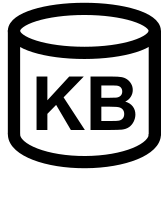
\includegraphics{../KB-symbol.png}}}}
\newcommand*\NewSym[2][0.5]{\vcenter{\hbox{\includegraphics[scale=#1]{#2}}}}
\newcommand*\sigmoid{\vcenter{\hbox{
\includegraphics{../sigmoid3.png}}}}
\newcommand{\smbox}[1]{\boxed{\footnotesize{\mbox{#1}}}}

\newcommand{\tikzmark}[1]{\tikz[overlay,remember picture] \node (#1) {};}

\newcommand{\Dfrac}[2]{%
\ooalign{%
      $\genfrac{}{}{2.9pt}0{\hphantom{#1}}{\hphantom{#2}}$\cr%
      $\color{white}\genfrac{}{}{1.5pt}0{\hphantom{#1}}{\hphantom{#2}}$\cr%
      $\color{white}\genfrac{}{}{1pt}0{\color{black}#1}{\color{black}#2}$}}

% \renewcommand{\thefootnote}{\fnsymbol{footnote}}
\usepackage{perpage}
\MakePerPage{footnote}
\renewcommand{\thefootnote}{\ifcase\value{footnote}\or{*}
	\or{$\dagger$}\or{**}\or{$\ddagger$}\fi}
\interfootnotelinepenalty=10000

\setlength{\parindent}{0pt}
\setlength{\parskip}{1.8ex plus0.8ex minus0.8ex}

% \usepackage[no-math]{fontspec}
% \setmainfont[BoldFont=Alibaba_Sans_Regular.otf,ItalicFont=Alibaba_Sans_Light_Italic.otf]{Alibaba_Sans_Light.otf}

\usepackage[backend=biber]{biblatex}
\bibliography{../AGI-book}

\usepackage[active,tightpage]{preview}		% for continuous page(s)
\renewcommand{\PreviewBorder}{0.5cm}
\renewcommand{\thempfootnote}{\arabic{mpfootnote}}

\usepackage[absolute,overlay]{textpos}		% for page number on upper left corner

\usepackage{color}
% \usepackage{mathtools}
\usepackage[hyperfootnotes=false]{hyperref}

% \usepackage[backend=biber,style=numeric]{biblatex}
% \bibliography{../AGI-book}
% \renewcommand*{\bibfont}{\footnotesize}

\usetikzlibrary{shapes}
% \usepackage[export]{adjustbox}	% ??
\usepackage{verbatim} % for comments
% \usepackage{newtxtext,newtxmath}	% Times New Roman font

% \titleformat{\subsection}[hang]{\bfseries\large\color{blue}}{}{0pt}{}
% \numberwithin{equation}{subsection}

\newcommand{\underdash}[1]{%
	\tikz[baseline=(toUnderline.base)]{
		\node[inner sep=1pt,outer sep=10pt] (toUnderline) {#1};
		\draw[dashed] ([yshift=-0pt]toUnderline.south west) -- ([yshift=-0pt]toUnderline.south east);
	}%
}%

\newcommand\reduline{\bgroup\markoverwith{\textcolor{red}{\rule[-0.5ex]{2pt}{0.4pt}}}\ULon}

%\DeclareSymbolFont{symbolsC}{U}{txsyc}{m}{n}
%\DeclareMathSymbol{\strictif}{\mathrel}{symbolsC}{74}
%\DeclareSymbolFont{AMSb}{U}{msb}{m}{n}
%\DeclareSymbolFontAlphabet{\mathbb}{AMSb}
%\setmathfont{lmroman17-regular.otf}
\DeclareMathOperator*{\argmin}{arg\,min}
\DeclareMathOperator*{\argmax}{arg\,max}

% \usepackage[most]{tcolorbox}
%\tcbset{on line,
%	boxsep=4pt, left=0pt,right=0pt,top=0pt,bottom=0pt,
%	colframe=red,colback=pink,
%	highlight math style={enhanced}
%}
%\newcommand{\atom}{\vcenter{\hbox{\tcbox{....}}}}

\let\oldtextbf\textbf
\renewcommand{\textbf}[1]{\textcolor{blue}{\oldtextbf{#1}}}

\newcommand{\logic}[1]{{\color{violet}{\textit{#1}}}}
\newcommand{\underconst}{
\includegraphics[scale=0.5]{../2020/UnderConst.png}}
\newcommand{\KBsymbol}{\vcenter{\hbox{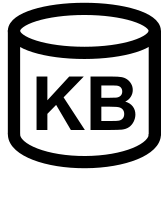
\includegraphics[scale=1]{../KB-symbol.png}}}}
\newcommand{\token}{\vcenter{\hbox{\includegraphics[scale=1]{token.png}}}}
\newcommand{\proposition}{\vcenter{\hbox{\includegraphics[scale=0.8]{proposition.png}}}}

\begin{document}

\begin{preview}

\title{\vspace{-1cm} \bfseries\color{blue}{\LARGE Future News - some ideas}}

\author{Yan King Yin} % Your name
% \date{\vspace{-2cm}} % Date, can be changed to a custom date

\centerline{
\includegraphics[scale=0.6]{Future-News-header.png}}

\maketitle

\setcounter{section}{-1}
\newcounter{mypage}
\setcounter{mypage}{0}

% (1) Circled page number on upper left corner
\begin{textblock*}{5cm}(2.1cm,2.3cm) % {block width} (coords)
{\color{red}{\large \textcircled{\small \themypage}}}
\addtocounter{mypage}{1}
\end{textblock*}

\begin{minipage}{\textwidth}
\setlength{\parskip}{0.4\baselineskip}

\begin{itemize}
	\item These are some of my suggested ideas, feel free to incorporate them

	\item I'm not forcing these ideas upon the team, but see if you agree or not...

	\item Basically I'm proposing 3 things:
	\begin{itemize}
			\item \textbf{Ranking mechanism}
			\item \textbf{Anti-racism}
			\item \textbf{DAO -- more even distribution of earnings}

	\end{itemize}
\end{itemize}

\end{minipage}
\end{preview}

\begin{preview}
\begin{textblock*}{5cm}(2.1cm,2.3cm) % {block width} (coords)
	{\color{red}{\large \textcircled{\small \themypage}}}
	\addtocounter{mypage}{1}
\end{textblock*}

\begin{minipage}{\textwidth}
	\setlength{\parskip}{0.4\baselineskip}

\section{Ranking mechanism}

\begin{itemize}
	\item News topics are diverse, we may lack experts to judge the quality of news items. Also, human judges may be \textbf{biased}.
	\item I suggest we should let news to ``\textbf{float}'' to the top via open public voting (ie, ``likes'')
	\item If content creators are at the top of their fields, they won't be afraid of competition.  Only scammers tend to confine their scope to gullible people, as more exposure works to their disadvantage.
\end{itemize}

\end{minipage}
\end{preview}

\begin{preview}
\begin{textblock*}{5cm}(2.1cm,2.3cm) % {block width} (coords)
{\color{red}{\large \textcircled{\small \themypage}}}
\addtocounter{mypage}{1}
\end{textblock*}

\begin{minipage}{\textwidth}
\setlength{\parskip}{0.4\baselineskip}

\section{Anti-racism}

\begin{itemize}
	\item Do Africans watch YouTube?  Yes.
	\item When people watch YouTube, traffic goes to YouTube, so do revenues.
	\item \textbf{Competition is global}, whether we're willing or unwilling.
	\item Generally speaking, we have to be \textbf{10$\times$ better} than YouTube to re-direct traffic to our site.  How is that possible?  Small, trivial features are insufficient.
	\item Currently there are some ``\textbf{black-hearted}'' software that are subtly racist.  For example, YouTube has the ability to mask your comments so others cannot see them, \textbf{without} the commenter knowing.  People who comment on YouTube may be talking into a black hole.  Another example:  ClubHouse has a feature that if just \textbf{one} member in a room dislikes you, you can be kicked out and unable to find that room, nor can you tell who kicked you out.  Such a feature means that \textbf{censorship} can be easily and anonymously achieved, which is especially useful to racist / bigotry groups.
	\item \textbf{Subtle racism} may look small and innocuous, but they are a \textbf{huge} thing.  Users who are pissed off will forever have a bitter feeling towards the black-hearted software.  This is where we can out-perform YouTube.
	\item Don't get me wrong -- I have friends in America and I love Americans.  But we cannot unconditionally love racists.  We have to \textbf{split} America into racists and non-racists -- that is critical to our \textbf{survival}.  It's either racists cry or racists make us cry.  Let it be the first option.
	\item USA is a very advanced country, they have freedom of speech and democracy.  YouTube also respects freedom of speech to a certain extent, but they do not have an explicit policy that guarantees that racial equality is upheld and that truthful comments will always not be banned.  That is our single most significant competitive advantage, IMO.  What if YouTube adopts the same policy as ours?  They can, in theory.  But America's \textbf{democracy works very slowly}.  For example, Israel is a racist, apartheid state but USA continues to support Israel with a double standard towards Palestinians.  It remains to be seen if the next president(s) will change the course of US foreign policy.  A similar situation may happen inside YouTube or other US corporations.  Their democracy may cause their products to be racist, due to their constituency, for at least quite some time to come.  That is the opportunity for us to make money.
	\item We have to \textbf{explicitly} state our anti-racist policy and the guarantee of no-banning of contents, and \textbf{well-publicize} this.  Users will feel the difference and be attracted to use our site.
	\item You may ask:  why would an \textbf{African} organization help fight global racism?  Why not just focus on Africa?  The same question applies to China, India, Iran, Russia, ... etc.  The problem is that if we all think our own country is ``\textbf{special}'' then we can never address the problem of racism and we will continue to live under racism and suffer from its oppression.  Everyone think they are ``special'' but then they become themselves racist and as bad as our oppressors.  And we won't win as long as we don't face the problem of racism.
	\item Some people of colored skin may get \textbf{angry} at my proposal because they think their suffering of racism was \textbf{greater}, and that by equalizing the \textbf{playing field} I am ignoring the differences of sufferance in different historical trajectories.  This is a complex issue that relates to making \textbf{reparations} for past events.  I am not making \textbf{pre-mature} conclusions on this.  Let's do things one at a time, and we can agree to creating a level playing field despite other complexities.
\end{itemize}

\end{minipage}
\end{preview}

\begin{preview}
\begin{textblock*}{5cm}(2.1cm,2.3cm) % {block width} (coords)
	{\color{red}{\large \textcircled{\small \themypage}}}
	\addtocounter{mypage}{1}
\end{textblock*}

\begin{minipage}{\textwidth}
	\setlength{\parskip}{0.4\baselineskip}

\section{DAO -- more even distribution of earnings}

\end{minipage}
\end{preview}

\end{document}
